%----------------------------------------------------------------------------------------
%	PACKAGES AND OTHER DOCUMENT CONFIGURATIONS
%----------------------------------------------------------------------------------------

\documentclass[idxtotoc,hyperref,openany]{article} % 'openany' here removes the gap page between days, erase it to restore this gap; 'oneside' can also be added to remove the shift that odd pages have to the right for easier reading

\usepackage[ 
  backref=page,
  pdfpagelabels=true,
  plainpages=false,
  colorlinks=true,
  bookmarks=true,
  pdfview=FitB]{hyperref} % Required for the hyperlinks within the PDF
  
\usepackage{booktabs} % Required for the top and bottom rules in the table
\usepackage{float} % Required for specifying the exact location of a figure or table
\usepackage{graphicx} % Required for including images
\usepackage{lipsum} % Used for inserting dummy 'Lorem ipsum' text into the template
\usepackage{enumitem}
\newcommand{\HRule}{\rule{\linewidth}{0.5mm}} % Command to make the lines in the title page
\setlength\parindent{0pt} % Removes all indentation from paragraphs
\usepackage[margin=1in]{geometry}
\usepackage{listings}
\usepackage{subfloat}
\usepackage{subcaption}
\lstset{
	numbers=left, 
	numberstyle=\small, 
	numbersep=8pt, 
	frame = single, 
	language=Pascal, 
	framexleftmargin=15pt}
%----------------------------------------------------------------------------------------
%	DEFINITION OF EXPERIMENTS
%----------------------------------------------------------------------------------------


%---------------------------------------------------------------------------------------

\begin{document}

%----------------------------------------------------------------------------------------
%	TITLE PAGE
%----------------------------------------------------------------------------------------

%\frontmatter % Use Roman numerals for page numbers
%\title{
%\begin{center}
%\HRule \\[0.4cm]
%{\Huge \bfseries Laboratory Journal \\[0.5cm] \Large Master of Science}\\[0.4cm] % Degree
%\HRule \\[1.5cm]
%\end{center}
%}
%\author{\Huge John Smith \\ \\ \LARGE john@smith.com \\[2cm]} % Your name and email address
%\date{Beginning 6 February 2012} % Beginning date
%\maketitle
%
%\tableofcontents
%
%\mainmatter % Use Arabic numerals for page numbers
%
%%----------------------------------------------------------------------------------------
%%	LAB BOOK CONTENTS
%%----------------------------------------------------------------------------------------
%
%% Blank template to use for new days:

%\labday{Day, Date Month Year}

%\experiment{}

%Text

%-----------------------------------------

%\experiment{}

%Text

%----------------------------------------------------------------------------------------

\title{EVN Primary Beam Model}
\date{Last updated: \today}
\author{Jack Radcliffe}
\maketitle




\section{Introduction}

This is the documentation for the primary beam model for the EVN developed by Jack Radcliffe as part of the Hubble Deep Field-North (HDF-N) wide-field VLBI project. Due to the lack of accurate primary beam models for many EVN telescopes, the primary beam can only be approximated as a Gaussian which is then applied directly to the upmost CL table in AIPS. To run the primary beam correction, you must have the packages described in Section 2.

%-----------------------------------------

\section{Requirements}

\begin{enumerate}[topsep=0pt,itemsep=-1ex,partopsep=1ex,parsep=1ex]
	\item Python version 2.7 (3+ is not supported) with packages:
	\begin{itemize}[topsep=0pt,itemsep=-1ex,partopsep=1ex,parsep=1ex]
		\item numpy
		\item astropy (version 1.3.3 is recommended, 2+ does not work at the moment, it is a known bug)
		\item scipy
		\item matplotlib
	\end{itemize}
	\item AIPS (31DEC16 or newer)
	\item ParselTongue 
	\item AIPS
\end{enumerate}
%\begin{figure}[H] % Example of including images
%\begin{center}
%\includegraphics[width=0.5\linewidth]{example_figure}
%\end{center}
%\caption{Example figure.}
%\label{fig:example_figure}
%\end{figure}

%-----------------------------------------

\section{Theory}

Each phase centre is primary beam corrected by following similar steps to Cao+2014. Due to the lack of accurate primary beam models for many EVN telescopes, the primary beam power response of each telescope were approximated by using a normalized, symmetric, 2D Gaussian of the form,

\begin{equation}
P(\theta, \phi) \approx \exp\left({\frac{(\theta- \theta_0)^2 + (\phi - \phi_0)^{2}}{2\sigma^2}}\right),
\end{equation}

\noindent where $P(\theta,\phi)$ is the relative power response. $\theta$ and $\phi$ are the respective azimuthal and polar angular distances from the antennas' pointing centers. The azimuthal and polar coordinates of the telescope's pointing centers are defined by $\theta_0$ and $\phi_0$ respectively. The standard deviation, $\sigma$, can be related to the FWHM of the primary beam, $\theta_{1/2}$, through the expression,

\begin{equation}
\sigma^2 = \frac{\theta_{1/2}^2}{8\ln{2}},
\end{equation} 

\noindent where the FWHM of the primary beam is defined as,
\begin{equation}
\theta_{1/2} = K\frac{\lambda_{\mathrm{c}}}{D_{\mathrm{eff}}}.
\end{equation}

\noindent Here, $\lambda_{\mathrm{c}}$, is the central wavelength of the observation and $D_{\mathrm{eff}}$ is the effective aperture diameter that takes into account any tapering of the telescope (Keimpema 2015, priv. comm.). The effective aperture diameters in use are shown in Table~\ref{table:telescopes}. A small correction factor, $K = 1.05$, is used to take into account any aperture blockages (Wrigley et al., in prep.). $P(\theta, \phi)$ was derived for each telescope at the centre of every phase centre. These correction factors are then applied using AIPS task \texttt{CLCOR}, where the gain amplitudes for each antenna were multiplied by the correction factors, $P(\theta, \phi)^{-1/2}$, of the two telescopes that form the baseline.

\begin{table}
	\centering  
	\begin{tabular}{lll}
		\hline\hline   \label{table:telescopes} 
		Telescopes & Country & Diameter (Effective)  \\
		\hline
		Ef & Germany & 100 (78) \\
		Wb & Netherlands & 25 \\
		On & Sweden & 25 \\
		Nt & Italy & 32 \\
		Tr & Poland & 32 \\
		Sv & Russia & 32 \\
		Bd & Russia & 32 \\
		Zc & Russia & 32 \\
		Sh & China & 25 (22.5)\\
		Jb1 & United Kingdom & 76 (67)\\
		\hline
		\noalign{\smallskip}
	\end{tabular}
	\caption{Sub-sample of EVN telescopes. Effective diameters are derived from fitting to beam models (A. Keimpema priv. comm.)}   
\end{table}
\section{Algorithm}

\begin{enumerate}[topsep=0pt,itemsep=-1ex,partopsep=1ex,parsep=1ex]
	\item \texttt{pbcor\_model.py} will take the inputs specified in this file and and uses \texttt{astropy.modeling} 2D Gaussians to model the primary beam shape. The standard deviation is entered as:
	\begin{eqnarray}
	\sigma_{\rm Dec} = (1/\cos({\rm Dec}))\frac{\theta_{1/2}}{(2\sqrt{2\log(2)})} \\
\sigma_{\rm RA} = \frac{\theta_{1/2}}{(2\sqrt{2\log(2)})}
	\end{eqnarray}
	
	and the full block of Python code implementing the model is:
	\begin{lstlisting}[basicstyle=\linespread{0.1},breaklines,language=Python]
	def station_HPBW(station,frequency):
		HPBW = ((constants.c/frequency)/station)*(180/np.pi)
		return HPBW
	
	xstd= station_HPBW(stations[telescope],frequency)/(2*np.sqrt(2*np.log(2)))*u.degree*(1/np.cos((phase_centers[i].dec.radian)))
	ystd =station_HPBW(stations[telescope],frequency)/(2*np.sqrt(2*np.log(2)))*u.degree
	models.Gaussian2D(amplitude=1, \
	x_mean=phase_centers[i].ra.degree,\
	y_mean=phase_centers[i].dec.degree,\
	x_stddev=xstd,\
	y_stddev=ystd, theta=0)
	\end{lstlisting}
	
	Examples of the Effelsberg (100m, effective 78m) and Medicina (32m) beams are shown in Figure~\ref{primary_beams}
	\begin{figure*}[t!]
		\centering
		\begin{subfigure}[t]{0.5\textwidth}
			\centering
			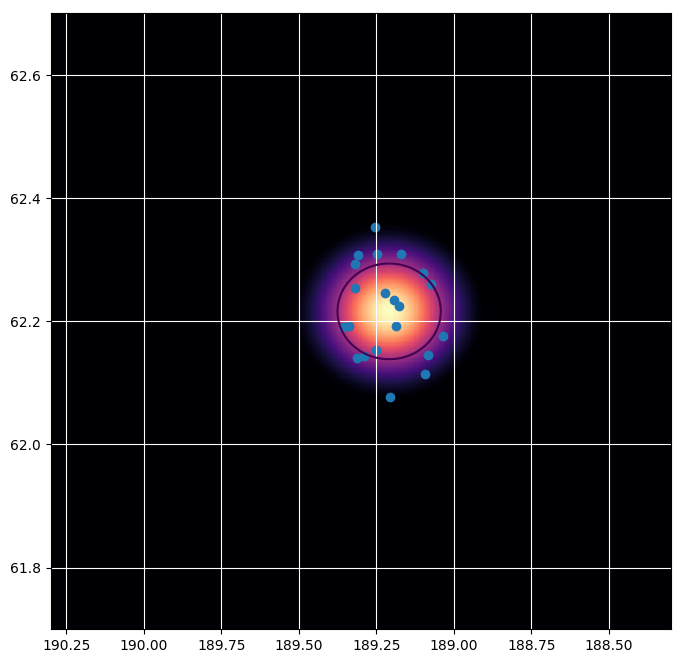
\includegraphics[height=.9\textwidth]{../PB_Plots/ROBLEDO_single_power_beam.png}
			\caption{Robledo 100m single power beam}
		\end{subfigure}%
		~ 
		\begin{subfigure}[t]{0.5\textwidth}
			\centering
			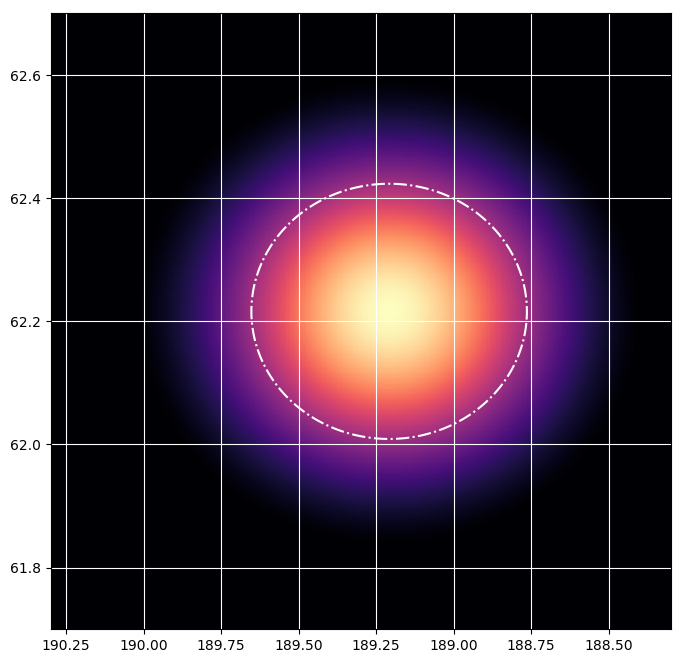
\includegraphics[height=.9\textwidth]{../PB_Plots/MEDICINA_single_power_beam.png}
			\caption{32m Medicina power beam}
		\end{subfigure}
		\caption{}
	\end{figure*}

	\item This code will then grid the model to the observational FoV (for either single or multiple pointings) and then use a user-defined number of FITS images to extract filenames and RA and Declinations. 
	
	\item These are evaluated per pointing and per telescope, where the square root is taken so that the value represents the **VOLTAGE** beam. This creates a \texttt{pickle} file which contains the corrections for each phase center and each telescope.
	
	\item \texttt{apply\_clcor\_Parseltongue.py} is then used to apply this to all the calibrated data sets. The data set (with only one phase centre) is moved to the current directory and the filename is checked against the filename of the fitsfiles (not pretty I know). The correction values for each telescope and pointing centre are parsed. The correction is applied to each telescope using AIPS Task \texttt{CLCOR} with \texttt{OPCODE='GAIN'}. This is applied to the upmost CL table. 
\end{enumerate}

\begin{figure}[H] % Example of including images
\begin{center}
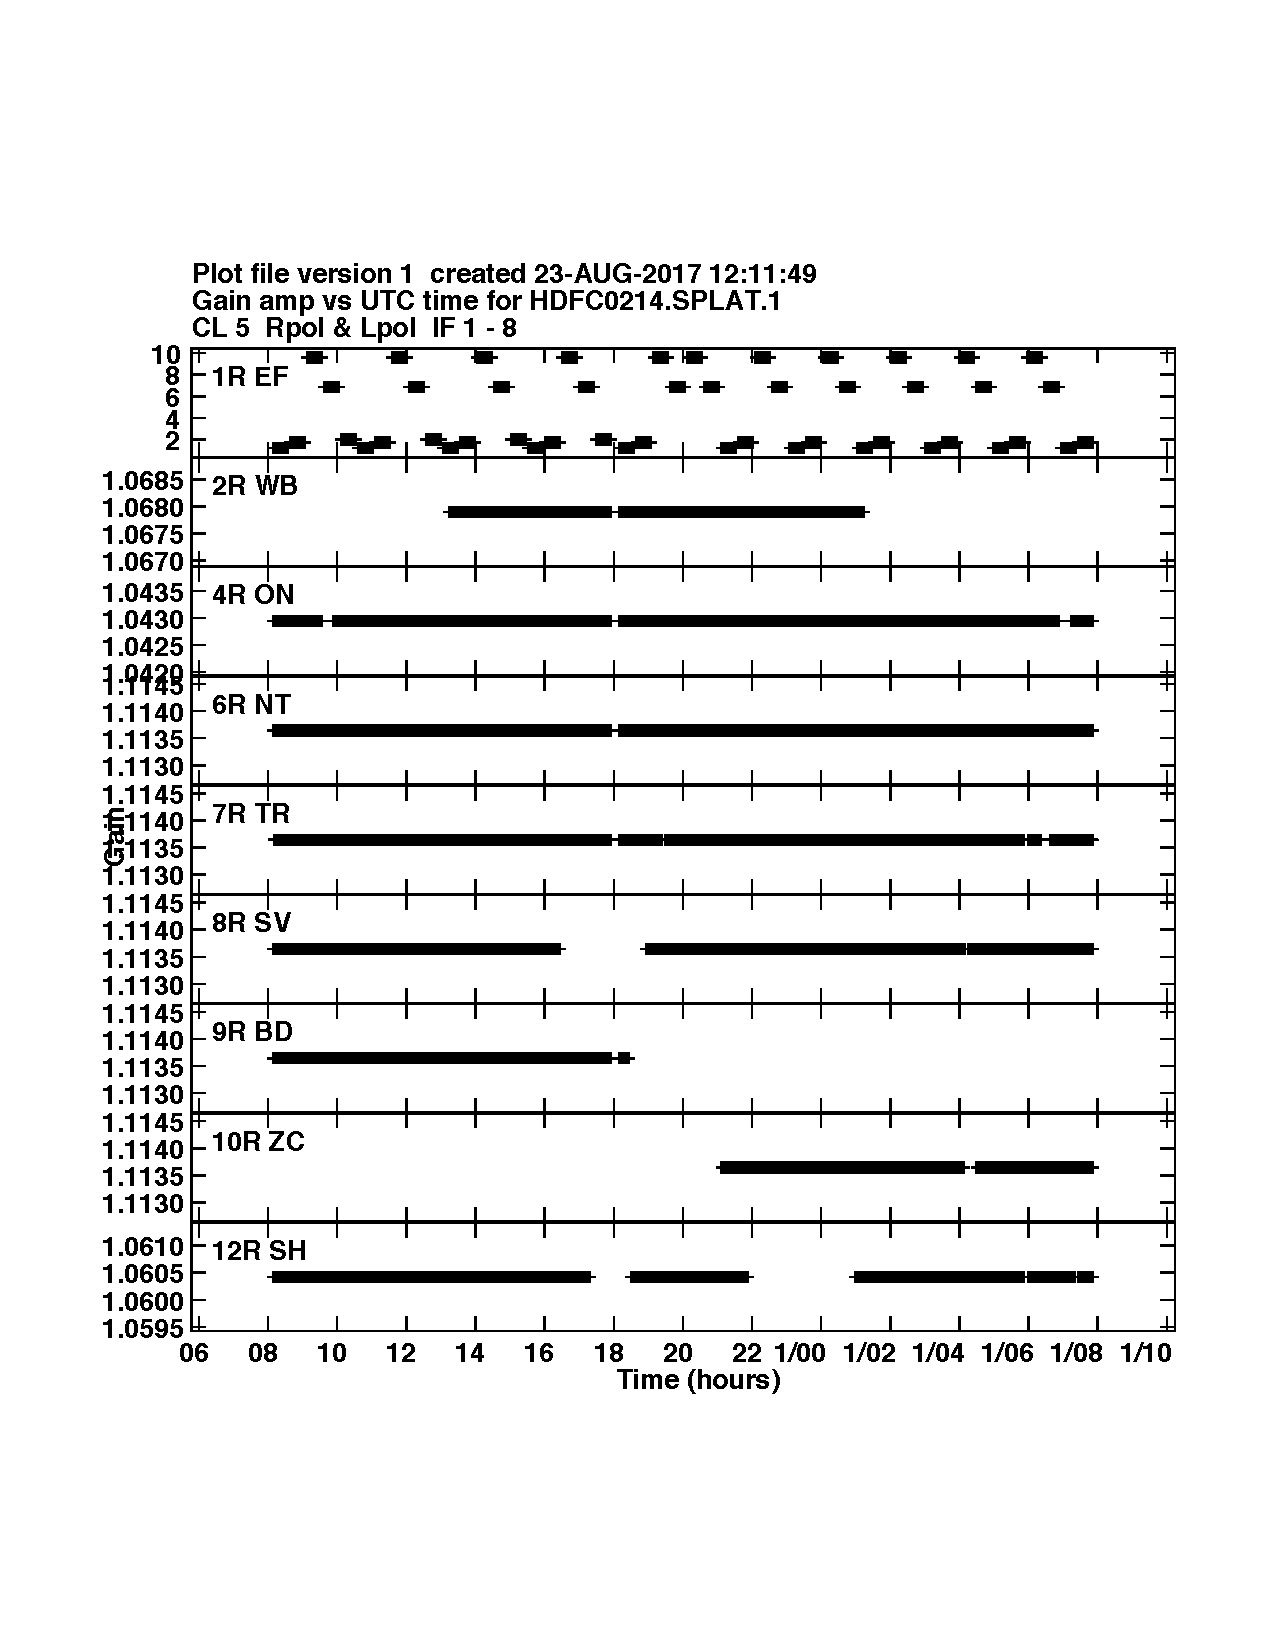
\includegraphics[page=1,width=\linewidth]{PBcor_CL_table.pdf}
\end{center}
\caption{CL table for HDF-N source HDFC0214. The EF telescope nods between 5 different pointings where three are close to the position of the source and 2 are distant $\sim$20arcmin. These furthest pointings are flagged in the observations subsequently as the primary beam model will diverge rapidly past the HPBW.}
\label{fig:example_figure}
\end{figure}

%%----------------------------------------------------------------------------------------
%
%\labday{Friday, 26 March 2010}
%
%\experiment{table}
%
%\begin{table}[H]
%\begin{tabular}{l l l}
%\toprule
%\textbf{Groups} & \textbf{Treatment X} & \textbf{Treatment Y} \\
%\toprule
%1 & 0.2 & 0.8\\
%2 & 0.17 & 0.7\\
%3 & 0.24 & 0.75\\
%4 & 0.68 & 0.3\\
%\bottomrule
%\end{tabular}
%\caption{The effects of treatments X and Y on the four groups studied.}
%\label{tab:treatments_xy}
%\end{table}
%
%Table \ref{tab:treatments_xy} shows that groups 1-3 reacted similarly to the two treatments but group 4 showed a reversed reaction.
%
%%----------------------------------------------------------------------------------------
%
%\labday{Saturday, 27 March 2010}
%
%\experiment{Bulleted list example} % You don't need to make a \newexperiment if you only plan on referencing it once
%
%This is a bulleted list:
%
%\begin{itemize}
%\item Item 1
%\item Item 2
%\item \ldots and so on
%\end{itemize}
%
%%-----------------------------------------
%
%\experiment{example}
%
%\lipsum[6]
%
%%-----------------------------------------
%
%\experiment{example2}
%
%\lipsum[7]
%
%%----------------------------------------------------------------------------------------
%%	FORMULAE AND MEDIA RECIPES
%%----------------------------------------------------------------------------------------
%
%\labday{} % We don't want a date here so we make the labday blank
%
%\begin{center}
%\HRule \\[0.4cm]
%{\huge \textbf{Formulae and Media Recipes}}\\[0.4cm] % Heading
%\HRule \\[1.5cm]
%\end{center}
%
%%----------------------------------------------------------------------------------------
%%	MEDIA RECIPES
%%----------------------------------------------------------------------------------------
%
%\newpage
%
%\huge \textbf{Media} \\ \\
%
%\normalsize \textbf{Media 1}\\
%\begin{table}[H]
%\begin{tabular}{l l l}
%\toprule
%\textbf{Compound} & \textbf{1L} & \textbf{0.5L}\\
%\toprule
%Compound 1 & 10g & 5g\\
%Compound 2 & 20g & 10g\\
%\bottomrule
%\end{tabular}
%\caption{Ingredients in Media 1.}
%\label{tab:med1}
%\end{table}
%
%%-----------------------------------------
%
%%\textbf{Media 2}\\ \\
%
%%Description
%
%%----------------------------------------------------------------------------------------
%%	FORMULAE
%%----------------------------------------------------------------------------------------
%
%\newpage
%
%\huge \textbf{Formulae} \\ \\
%
%\normalsize \textbf{Formula 1 - Pythagorean theorem}\\ \\
%$a^2 + b^2 = c^2$\\ \\
%
%%-----------------------------------------
%
%%\textbf{Formula X - Description}\\ \\
%
%%Formula
%
%%----------------------------------------------------------------------------------------
%
\end{document}